\begin{figure}[h]
    \centering
    \begin{tabular}{m{1.5cm}m{1.5cm}m{1.5cm}m{0.4cm}m{0.5cm}}
    %   \hline

    %   \multirow{2}{*}{Input} &  (i) & (ii) & (iii) & (iv) & (v) & (vi) \\
    %   &  CA guidance &  $\vz_t$  guidance & SA replace.&  SA guidance &   (iv)+CA replace. &  (v) + LB \\
      %& \centering  CA guidance & \centering  $\vz_t$  guidance & \centering  SA replace.& \centering : SA guidance & \centering  (iv)+CA replace. & \centering  (v) + LB \\
    %   \hline
    %   \multicolumn{7}{c}{``\textit{a girl with blonde hair \textcolor{RoyalBlue}{\textbf{and a fluffy rainbow hat}} smiling}"} \\
    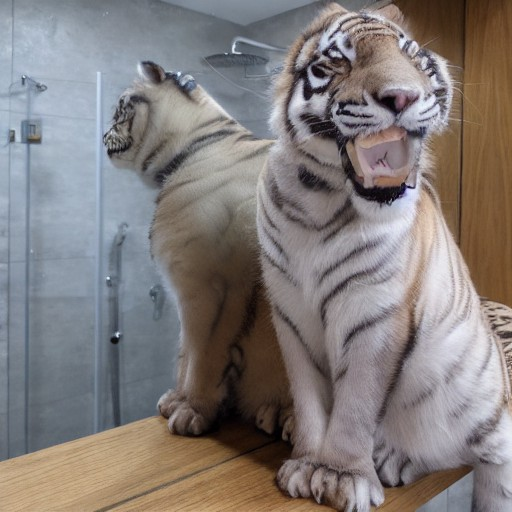
\includegraphics[width=1.5cm]{fig/cfg_self_matrix/m_2_50} & 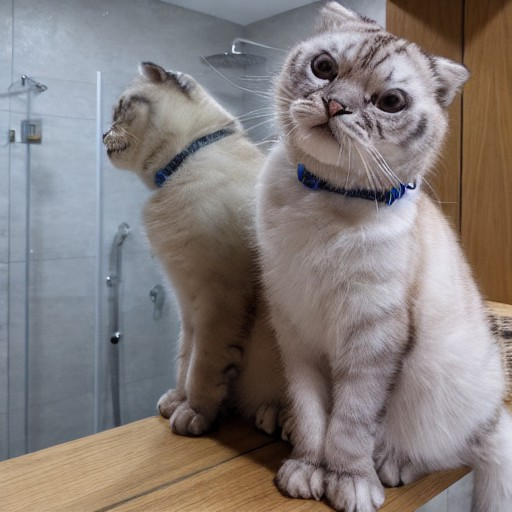
\includegraphics[width=1.5cm]{fig/cfg_self_matrix/m_2_250} & 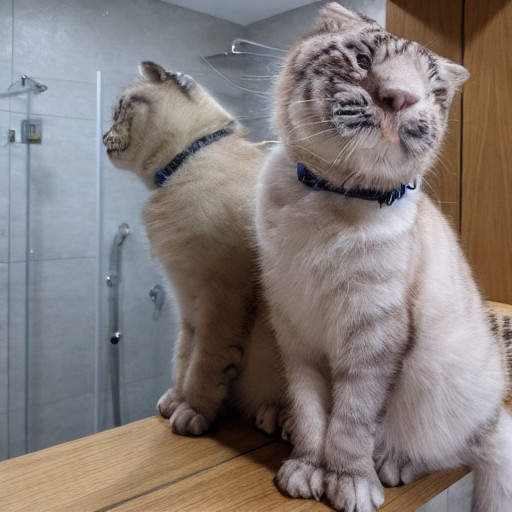
\includegraphics[width=1.5cm]{fig/cfg_self_matrix/m_2_500} & \rotatebox[origin=c]{90}{$w=2$} & \multirow{3}{*}{\rotatebox[origin=c]{90}{\textit{Classifier-Free guidance}}} \\
    
    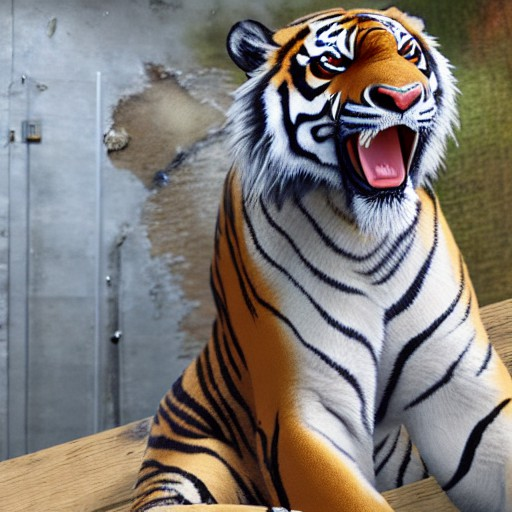
\includegraphics[width=1.5cm]{fig/cfg_self_matrix/m_75_50} & 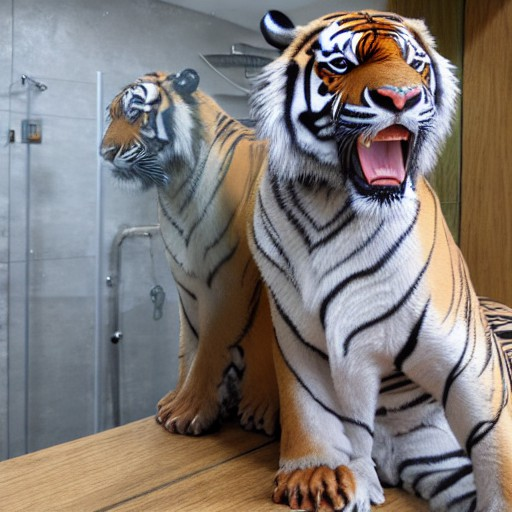
\includegraphics[width=1.5cm]{fig/cfg_self_matrix/m_75_250} & 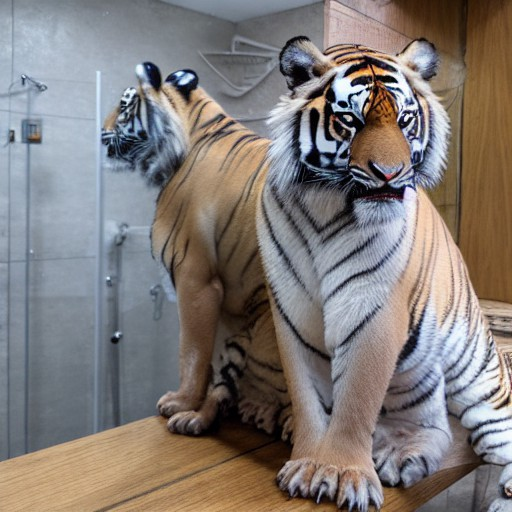
\includegraphics[width=1.5cm]{fig/cfg_self_matrix/m_75_500} & \rotatebox[origin=c]{90}{$w=7.5$} &  \\
    %   \multicolumn{7}{c}{``\textit{a baby with a stuffed \textcolor{BrickRed}{\st{monkey}} \textcolor{RoyalBlue}{\textbf{zebra}} in a car}"} \\
    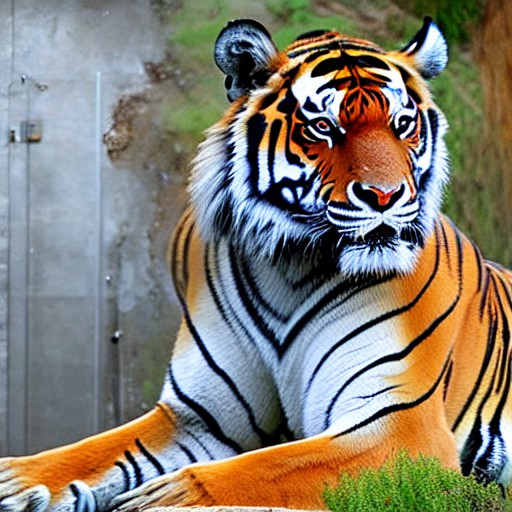
\includegraphics[width=1.5cm]{fig/cfg_self_matrix/m_15_50} & 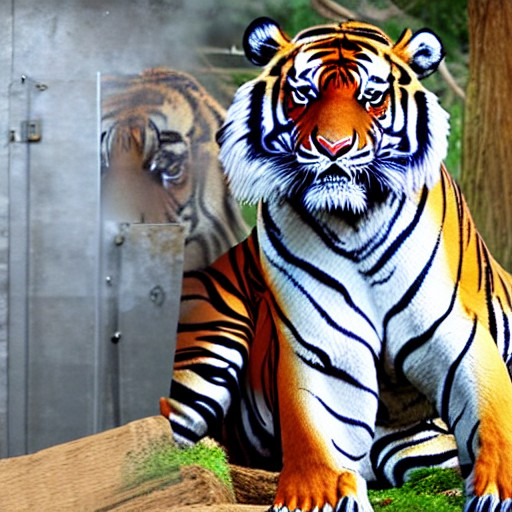
\includegraphics[width=1.5cm]{fig/cfg_self_matrix/m_15_250} & 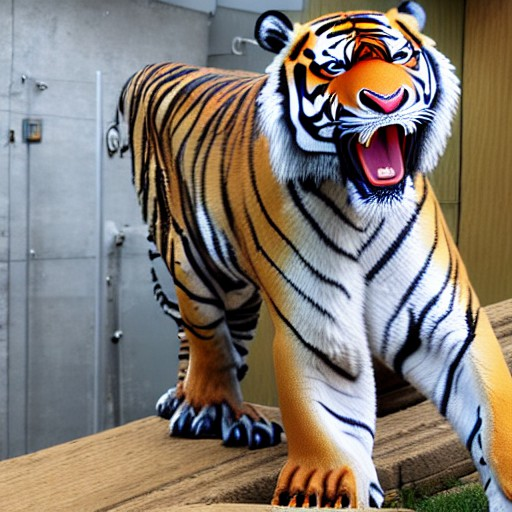
\includegraphics[width=1.5cm]{fig/cfg_self_matrix/m_15_500} & \rotatebox[origin=c]{90}{$w=15$} &  \\
    \centering  $ \lambda = 50 $  & \centering  $ \lambda = 250 $ & \centering  $ \lambda = 500 $ & & \\
    \multicolumn{3}{c}{\textit{Self-attention guidance}} & & \\
      % ... Add more rows as needed
    \end{tabular}
    % \caption{Matrix showing CFG $w$ and self-attention guidance scale $\lambda$ and how each of them drives the image generation toward reconstruction (high $\lambda$ and low $w$) or editing (low $\lambda$ and high $w$). Prompt: ``\textit{a \textcolor{BrickRed}{\st{cat}} \textcolor{RoyalBlue}{\textbf{tiger}} sitting next to a mirror}"}
    \caption{This matrix illustrates the interplay between CFG $w$ and self-attention guidance scale $\lambda$, highlighting their influence on image generation. The matrix shows how varying levels of $\lambda$ and $w$ drive the generated image toward either reconstruction (achieved with high $\lambda$ and low $w$) or editing (achieved with low $\lambda$ and high $w$). The images are generated based on the prompt ``'\textit{a \textcolor{BrickRed}{\st{cat}} \textcolor{RoyalBlue}{\textbf{tiger}} sitting next to a mirror}''.}
    \label{fig:supablation_cfg_guidance}
  \end{figure}